\section{Rozkład według wartości osobliwych}\label{sec:compression_svd}

Drugim algorytmem który postanowiliśmy sprawdzić badając kompresję obrazu
był rozkład według wartości osobliwych (SVD - singular value decomposition).
Jeśli każdy piksel potraktujemy jako pojedyńczą wartość (np w skali szarości,
lub systemu pozycyjnego o podstawie 255), to rozkład macierzy pikseli na wartości
osobliwe spowoduje wydzielenie z niech cech bardziej i mniej charakterystycznych,
ponieważ początkowe wartości osobliwe kodują najwięcej informacji. Następnie można
odtworzyć macierz dodając do siebie jedynie część wartości osobliwych. Wówczas zdjęcie
zredukuje swój rozmiar, jednocześnie zachowując najważniejsze szczegóły.

Obrazek testowy poniżej miał 512x512 pikseli, więc możliwe było podzielenie go na 512
wartości osobliwych. W wynikach możemy dostrzec poprawiającą się jakość wraz z rozmiarem
i liczbą wartości osobliwych wziętych pod uwagę. Ciekawym efektem który możemy zaobserwować
w przypadku formatu png, jest spadek rozmiaru przy wszystkich 512 wartościach osobliwych.

\begin{center}
    \begin{longtable}{|l|c|c|}
        \caption{Porównanie przebiegów}\\
        \hline
        \textbf{\thead{Ilość wartości \\ osobliwych}} & \textbf{JPG} & \textbf{PNG} \\
        \hline
        \endfirsthead
        \multicolumn{3}{c}%
        {\tablename\ \thetable\ -- \textit{cd}} \\
        \hline
        \textbf{\thead{Ilość wartości \\ osobliwych}} & \textbf{JPG} & \textbf{PNG} \\
        \hline
        \endhead
        \multicolumn{3}{r}{\textit{cdn}} \\
        \endfoot
        \endlastfoot

        \hline
        org & 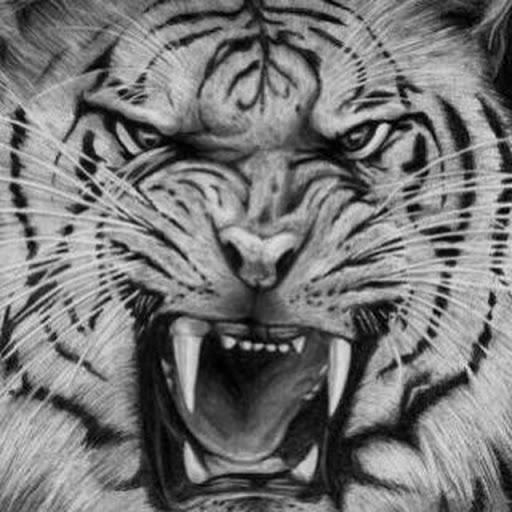
\includegraphics[width=0.4\textwidth]{photos/photo_org.jpg} & 
\includegraphics[width=0.4\textwidth]{photos/photo_org.png} \\
        & 46K & 247K \\
        \hline
        1 & 
\includegraphics[width=0.4\textwidth]{photos/photo_1.jpg} & 
\includegraphics[width=0.4\textwidth]{photos/photo_1.png} \\
        & 14K & 363K \\
        \hline
        5 & 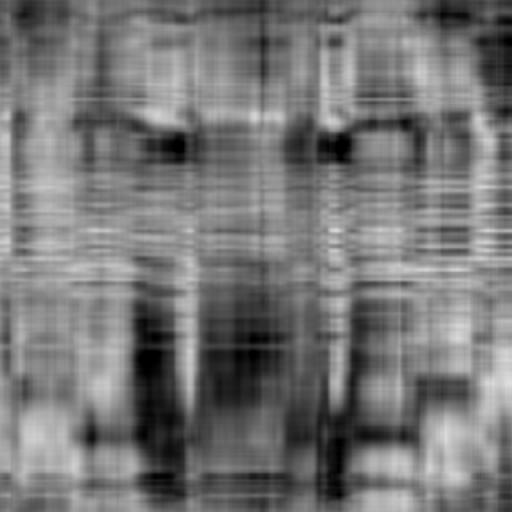
\includegraphics[width=0.4\textwidth]{photos/photo_5.jpg} & 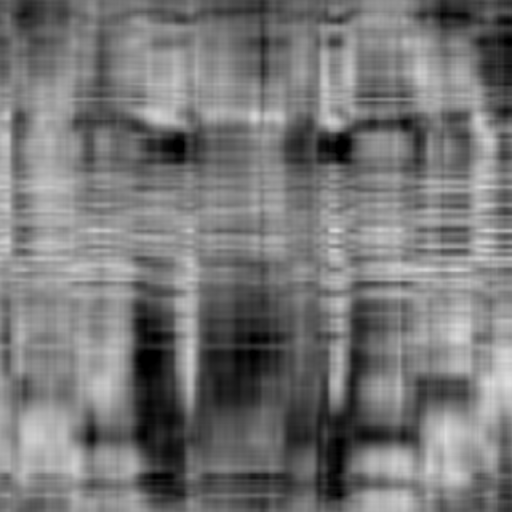
\includegraphics[width=0.4\textwidth]{photos/photo_5.png} \\
        & 21K & 411K \\
        \hline
        10 & 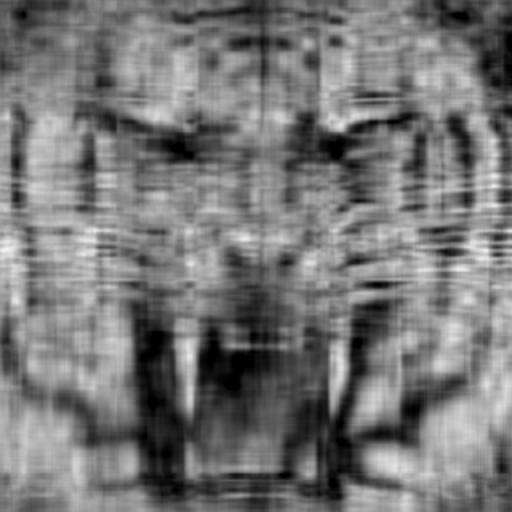
\includegraphics[width=0.4\textwidth]{photos/photo_10.jpg} & 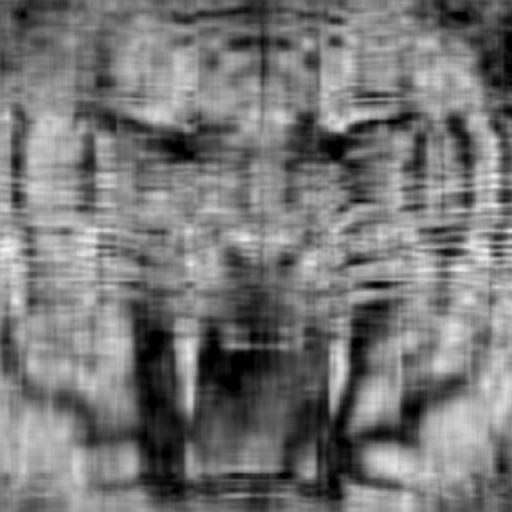
\includegraphics[width=0.4\textwidth]{photos/photo_10.png} \\
        & 26K & 429K \\
        \hline
        15 & 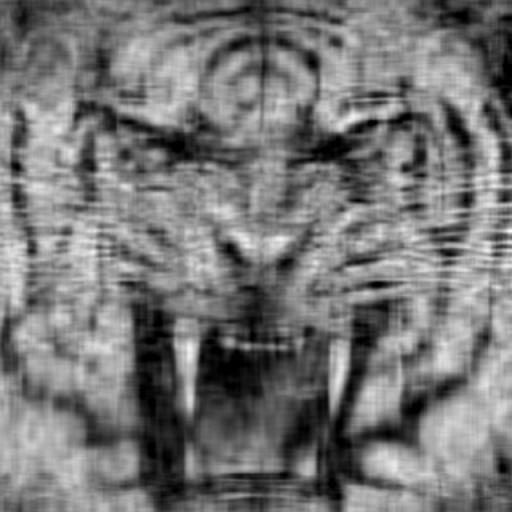
\includegraphics[width=0.4\textwidth]{photos/photo_15.jpg} & 
\includegraphics[width=0.4\textwidth]{photos/photo_15.png} \\
        & 29K & 438K \\
        \hline
        50 & 
\includegraphics[width=0.4\textwidth]{photos/photo_50.jpg} & 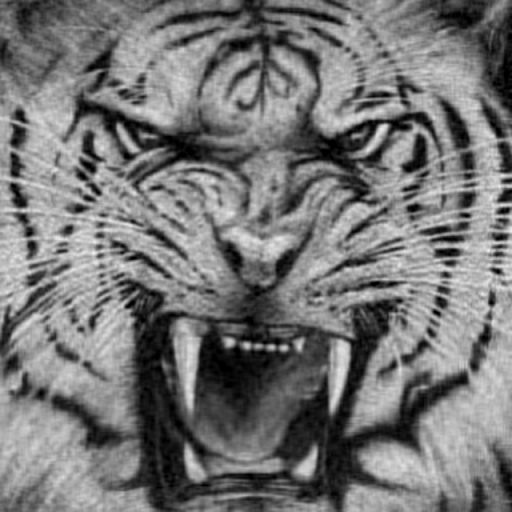
\includegraphics[width=0.4\textwidth]{photos/photo_50.png} \\
        & 39K & 456K \\
        \hline
        100 & 
\includegraphics[width=0.4\textwidth]{photos/photo_100.jpg} & 
\includegraphics[width=0.4\textwidth]{photos/photo_100.png} \\
        & 44K & 464K \\
        \hline
        512 & 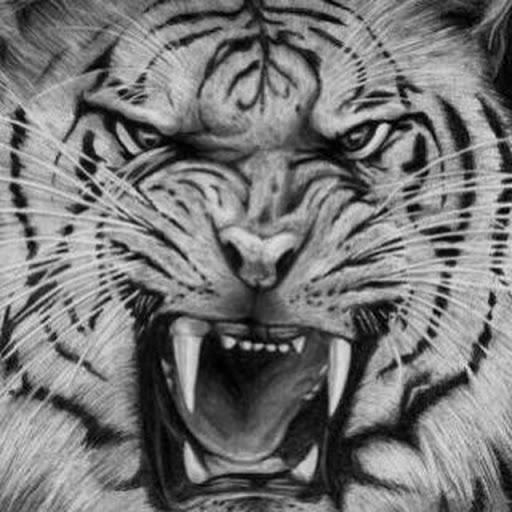
\includegraphics[width=0.4\textwidth]{photos/photo_512.jpg} & 
\includegraphics[width=0.4\textwidth]{photos/photo_512.png} \\
        & 46K & 247K \\
        \hline
    \end{longtable}
\end{center}

Niestety zadawalająca jakość obrazu pojawia się przy ok 20\% oryginalnego obrazu, co daje zmniejszenie
rozmiaru w granicach 5\%. Spadek jakości jest zauważalny i ta numeryczna metoda kompresji nie oferuje
wystarczającego zmniejszenia rozmiaru przy tak znaczącym spadku jakości. Dlatego też ją także odrzuciliśmy.
